\chapter{Neural Networks for NLP}

Neural networks are \textbf{universal function approximators} that can learn complex patterns in data. They have become a cornerstone of modern natural language processing (NLP) due to their ability to model the intricacies of human language. In this chapter, we will explore the fundamental concepts of neural networks and how they are applied in NLP tasks. In theory, just \textbf{one hidden layer} is sufficient to approximate any function (very very large though), but in practice, deeper networks often yield better performance.
This is also true if we require hidden layers to be of fixed size $N$ but we allow for arbitrary depth $D$. 

Why are we using neural networks?
\begin{enumerate}
    \item They go beyond the so called \textbf{feature engineering} paradigm, where we manually design features to represent the data. Neural networks can automatically learn relevant features from raw data, reducing the need for extensive feature engineering;
    \item Inner layers construct \textbf{meaningful representations} of the data, only from raw inputs (+ labels).
\end{enumerate}

\section{Basic Concepts of Neural Networks}

We start from a vector of inputs:
\[
x \in \mathbb{R}^n
\]
and we want to predict a vector of outputs:
\[
y = f(z_x) = f(w\cdot x + b) 
\]
where:
\begin{itemize}
    \item $w \in \mathbb{R}^m$ is a weight vector;
    \item $b \in \mathbb{R}$ is a bias term;
    \item $f$ is a non-linear activation function.
\end{itemize}

\begin{center}
    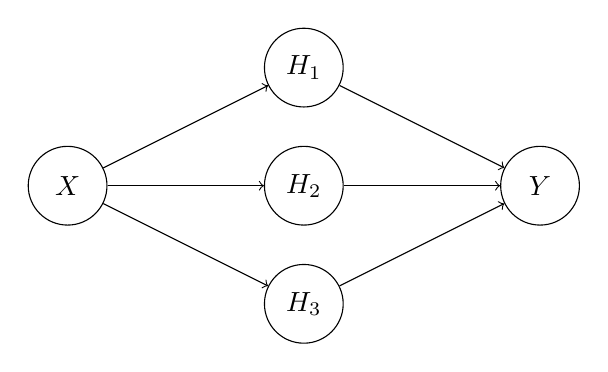
\begin{tikzpicture}[x=2cm, y=1.5cm, every node/.style={circle, draw, minimum size=1cm}]
        % Input layer (3 neurons)
        \node[] (X) at (0,-2) {$X$};
        
        % Hidden layer (3 neurons)
        \foreach \j in {1,...,3} {
            \node[] (H\j) at (1.5,-\j) {$H_{\j}$};
        }
        
        % Output layer (1 neuron)
        \node[] (Y1) at (3,-2) {$Y$};
        
        % Connect input layer to hidden layer
        \foreach \j in {1,...,3} {
            \draw[->] (X) -- (H\j);
        }
        
        % Connect hidden layer to output layer
        \foreach \i in {1} {
            \foreach \j in {1,...,3} {
                \draw[->] (H\j) -- (Y\i);
            }
        }
    \end{tikzpicture}
\end{center}

The \textbf{activation function} $f$ introduces non-linearity into the model, allowing it to learn complex patterns. Common activation functions include:
\begin{itemize}
    \item \textbf{ReLU} (Rectified Linear Unit): $f(z) = \max(0, z)$
    \item \textbf{Sigmoid}: $f(z) = \frac{1}{1 + e^{-z}}$
\end{itemize}

\begin{warningblock}
    Due to \textbf{asymptotic properties}, ReLU is generally preferred over Sigmoid in hidden layers, as it helps mitigate the vanishing gradient problem and allows for faster training.
\end{warningblock}

XOR is the classical example of a function that is not linearly separable, meaning that it cannot be represented by a single linear decision boundary. A neural network with at least one hidden layer can learn to represent the XOR function by combining multiple linear decision boundaries in a non-linear way.

\begin{quote}
    There is a depth 2 NN with ReLU activation that approximates XOR.
\end{quote}
\begin{flushright}
    -- GOODFELLOW (2016)
\end{flushright}

\missing{graphs for AND, OR, XOR and the NN for XOR}

Multiplying by the matrix 
\[
W = \begin{bmatrix}1 & 1 \\ 1 & 1 \end{bmatrix}
\]
added to the bias $b = \begin{bmatrix}0 \\ -1\end{bmatrix}$ and then applying ReLU, we get a linearly separable space.

\section{Feedforward Neural Networks}

There are problems with classical NN:
\begin{itemize}
    \item Leave the choice of non-linearity;
    \item Hidden representation can have arbitrary dimension and we want arbitraty number of layers;
    \item Dimension of output can vary depending on the number of classes;
    \item We want outputs to be \textbf{probabilities}.
\end{itemize}

Starting with the fourth point, we can use the \textbf{softmax} function to convert raw output scores (logits) into probabilities. The softmax function is defined as:
\[
\text{softmax}(z_i) = \frac{e^{z_i}}{\sum_{j} e^{z_j}}
\]
where $z_i$ is the $i$-th element of the input vector $z$. This ensures that the output values are in the range (0, 1) and sum to 1, making them interpretable as probabilities.

\begin{tipsblock}[Exponential function]
    Why the exponential? It is \textbf{monotonic}, \textbf{non-negative} and \textbf{good for derivative}.
\end{tipsblock}

The parameters in the network are \textbf{weights} and \textbf{biases}, which are learned during training. First of all, we need data:
\[
X_{train} = \left\{(x_1, y_1), (x_2, y_2), \ldots, (x_n, y_n)\right\}, \quad X_{test} = \left\{(x_1, y_1), (x_2, y_2), \ldots, (x_m, y_m)\right\}
\]

We define a \textbf{loss function} $L(y, \hat{y})$ that measures the difference between the predicted output $\hat{y}$ and the true output $y$. At a certain point we will have 
\[
\underbar{y} = softmax(\hat{y}), \quad \hat{y} \in \left\{0,1,\dots,C\right\}
\]
and we can use the \textbf{cross-entropy loss} for multi-class classification:
\[
L(y, \hat{y}) = -\sum_{i=1}^{C} y_i \log(\hat{y}_i)
\]

The goal of training is to minimize the loss function over the training data by adjusting the weights and biases in the network. This is typically done using optimization algorithms such as \textbf{Stochastic Gradient Descent} (SGD) or its variants (e.g., Adam, RMSprop). 
We approach stochasticity by using \textbf{mini-batches}, small random subsets of the training data, to compute the gradients and update the parameters. This helps to reduce the variance in the updates and can lead to faster convergence.

\begin{exampleblock}[Wrong sentiment classification with NN]
    We have a \textit{Corpus} $\mathcal{C}$, i.e. a collection of tweets, and we want to classify them as \textit{positive}, \textit{negative} or \textit{neutral}.
    \[
    \mathcal{C}_{train} = \left\{(x_1, y_1), (x_2, y_2), \ldots, (x_n, y_n)\right\}, \quad \mathcal{C}_{test} = \left\{(x_1, y_1), (x_2, y_2), \ldots, (x_m, y_m)\right\}
    \]
    where $x_i$ is a tweet and $y_i \in \{\text{positive}, \text{negative}, \text{neutral}\}$.
    The \textbf{idea} is to convert each tweet into a vector of features and then feed it into a neural network for classification.
    \begin{itemize}
        \item $x_1 = \log (\text{count of tokens})$
        \item $x_2 =$ \# of \textbf{bad} tokens
        \item $x_3 =$ \# of \textbf{good} tokens
        \item $x_4 = \begin{cases} 1 & \text{if 'no' in tweet} \\ 0 & \text{otherwise} \end{cases}$
        \item $x_5 = \begin{cases} 1 & \text{if '?' in tweet} \\ 0 & \text{otherwise} \end{cases}$
        \item $x_6 =$ count of $1^{st}$ person pronouns
    \end{itemize}
    The problem is that this model \textbf{will not perform well}.
\end{exampleblock}

\textbf{One-Hot-Encoding} is a way to represent categorical variables as binary vectors. Each category is represented by a vector of length equal to the number of categories, with a 1 in the position corresponding to the category and 0s elsewhere. For example, if we have three categories: \textit{cat}, \text{dog}, and \textit{bird}, we can represent them as:
\[
\text{cat} = [1, 0, 0], \quad \text{dog} = [0, 1, 0], \quad \text{bird} = [0, 0, 1]
\]

It follows the tokenization of the corpus:
\[
\mathcal{C} = \text{corpus} \rightarrow^{tokenization (BPE)} \mathcal{V} = \text{vocaboulary} \rightarrow^{OHE} \text{vector} \in \mathcal{R}^{|\mathcal{V}|}
\]

\begin{observationblock}
    Input is in $\mathcal{R}^{|\mathcal{V}|\cdot n}$. The $n$ is \textbf{variable} and depends on the number of tokens in the tweet. There are different solutions:
    \begin{itemize}
        \item \textbf{Pad} the input to a fixed length (e.g., 50 tokens) and truncate longer tweets. This allows us to have a fixed-size input vector, but it may lead to loss of information for longer tweets.
        \item \textbf{Cut} the input into fixed-size chunks (e.g., 10 tokens each) and process each chunk separately. This allows us to handle variable-length inputs, but it may lead to loss of context between chunks.
        \item \textbf{Average} the embeddings of all tokens in the tweet to obtain a fixed-size vector. This allows us to capture the overall meaning of the tweet, but it may lose information about the order of tokens.
    \end{itemize}
    They will return an \textbf{Embedding}, a dense vector representation of the input text, which can be fed into the neural network.
\end{observationblock}

